\chapter{Análisis Experimental}
Este capítulo presenta la evaluación experimental del AE multiobjetivo propuesto para resolver el problema de sincronización de semáforos en el Corredor Garzón. Inicialmente se presenta una descripción de los escenarios utilizados en la evaluación experimental y la plataforma de ejecución en la que se llevó a acabo la experimentación. A continuación se detalla el análisis experimental, que se divide en dos etapas: primero se analiza la configuración paramétrica inicial del AE con el objetivo de obtener una mejor calidad de resultados y luego se realizan los experimentos de validación para los que se reportan los resultados numéricos. Finalmente se ofrece un breve análisis de la eficiencia computacional del AE propuesto.



\section{Plataforma de ejecución y Desarrollo}

Dada la complejidad del problema, el análisis experimental se realiza en la infraestructura computacional de alto desempeño Cluster Fing (http://www.fing.edu.uy/cluster) con el objetivo de acelerar el tiempo real de procesamiento al ejecutar el AE en paralelo. De esta forma se distribuye la carga de procesamiento en varios núcleos. El cluster Fing cuenta con procesadores AMD Opteron 6272 de 2.09GHz, 48Gb RAM, 64 núcleos, con sistema operativo CentOS Linux 6.5.

Las pruebas incluidas en el análisis experimental utilizaron entre 4 y 32 núcleos de procesamiento. Dada la naturaleza de recursos compartidos del Cluster, no siempre es posible contar con la misma cantidad de recursos disponibles, además, para la mayoría de las pruebas el número de núcleos no es relevante. El numero de núcleos utilizados será tenido en cuenta, cuando se realice el análisis de eficiencia computacional detallado al final de este capítulo.


\section{Ajuste paramétrico}
Se realiza un análisis previo para determinar el mejor valor de los parámetros del AE propuesto. Este análisis tiene como objetivo obtener una mejor calidad de resultados. Los parámetros que se ajustan incluyen el \emph{tiempo de simulación} que se refiere al parámetro del simulador SUMO para determinar la duración de la simulación. Luego el \emph{criterio de parada} que indica el método usado para detener el algoritmo y el \emph{tamaño de la población} que representa la cantidad de individuos de la población utilizada en el AE. Finalmente se ajustan los parámetros de \emph{probabilidad de mutación y probabilidad de cruzamiento}. Estos parámetros serán descritos en detalle en las siguientes secciones.

Para comenzar el análisis del ajuste paramétrico se generan tres escenarios de tráfico diferentes. Estos escenarios no incluyen datos recabados de la realidad (como el tráfico vehicular o la frecuencia de los ómnibus), para no ajustar los parámetros a un caso particular.
A continuación se presenta la cantidad de vehículos para cada uno de los tres escenarios de tráfico propuestos:

\begin{itemize}
	\item Tráfico Bajo: 30 ómnibus y 500 vehículos	
	\item Tráfico Medio: 60 ómnibus y 1000 vehículos
	\item Tráfico Alto: 120 ómnibus y 2000 vehículos
\end{itemize}


En el ajuste paramétrico los primeros parámetros que se definen son: el tiempo de simulación, el criterio de parada y el tamaño de población. Luego de establecidos los valores para los parámetros mencionados, se realizan las pruebas para todas las combinaciones de probabilidad de cruzamiento y mutación buscando los valores con los cuales el AE obtiene una mejor calidad de resultados.

%La plataforma Cluster Fing donde se desarrolla el análisis experimental permite disponer tanto de la métrica del tiempo real que dura la ejecución, así como también el tiempo secuencial, es decir la suma del tiempo de procesamiento de todos los procesadores involucrados en la evaluación del algoritmo. Cuando se realizan comparaciones en los tiempos de ejecución se utiliza el tiempo secuencial que es independiente de la cantidad de procesadores utilizados en las pruebas. 

\subsection{Pesos de la función de fitness}

Para el análisis experimental la función \emph{fitness} del algoritmo (\ref{eq:funcion_fitness}) tendrá los pesos \emph{$w_1$ = $w_2$ = 1}. Estos valores dan pesos equitativos tanto a ómnibus como a otros vehículos, por lo que no existe prioridad para uno u otro. Más adelante se realizarán experimentos con otras variantes.


\subsection{Tiempo de simulación}
El tiempo de simulación refiere a la duración de la ejecución de una simulación usando SUMO. Es un parámetro que se puede configurar y permite tener un mejor control sobre los tiempos totales de ejecución del algoritmo.

Se establece un tiempo de simulación de 4000 \emph{steps} (medida interna de tiempo del simulador). Este número representa 66 minutos en la simulación, mientras que el tiempo real de ejecución depende de la plataforma computacional utilizada y de la cantidad de vehículos considerados en el escenario. En las simulaciones realizadas en el marco de este proyecto se encuentra entre los 5 y 20 segundos. En el análisis experimental se tuvo en cuenta y validó que en cada escenario más del 80 \% de los vehículos completaran la simulación, es decir que llegaran a sus destinos. Se realizaron 10 ejecuciones del AE para cada uno de los tres tipos de tráfico, comprobando que se cumplía el criterio anterior.


\subsection{Criterio de parada}
Se elige como criterio de parada un determinado número de generaciones. Este criterio permite estandarizar las pruebas y evaluar una comparación justa entre los distintos escenarios de tráfico. Para determinarlo, se busca un compromiso entre un buen resultado numérico y un tiempo de ejecución que no sea excesivo. Se determina que esta duración se encuentre entre 1 y 24 horas, y para potencialmente obtener un buen resultado numérico se comprueba experimentalmente que el valor de \emph{fitness} no presente variaciones importantes en las últimas 100 generaciones.  

Para determinar este criterio se realizaron 10 ejecuciones del AE por cada uno de los tres tipos de tráfico, eligiendo el número de 500 generaciones como criterio de parada. En la Figura \ref{fig:criterio_parada} se aprecia como el valor de \emph{fitness} no presenta grandes variaciones luego de la generación 400, además el tiempo de ejecución real se encuentra dentro del margen pautado. La gráfica no muestra todos los valores obtenidos, sólo algunos valores representativos para una mejor visualización.

\begin{figure}[h]
\centering
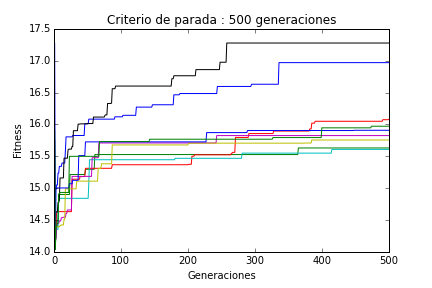
\includegraphics[width=0.8\linewidth]{Figures/criterio_parada}
\caption[Gráfica de la evolución de los valores de fitness. ]{Gráfica de la evolución de los valores de fitness para establecer el criterio de parada.}
\label{fig:criterio_parada}
\end{figure}

\subsection{Tamaño de la población}

Para la elección del tamaño de la población se tienen en cuenta tres elementos: el valor de \emph{fitness} resultante de la ejecución del AE, el tiempo de ejecución total y los recursos de la plataforma de ejecución.

La máxima cantidad poblacional a estudiar está determinada por la infraestructura del Cluster Fing, donde la cantidad máxima de núcleos en el mismo nodo es de 64. Teniendo en cuenta que la mejor distribución de trabajo es un individuo por núcleo, se determina que la máxima cantidad de individuos en la población será de 64. Luego se establecen dos valores más para completar el análisis, con un tamaño de población de 32 y 48 individuos. Se eligen estos valores ya que no son lo suficientemente bajos y se logra una distribución adecuada de individuos en la infraestructura.

La Tabla \ref{table:parametro_poblacion} muestra los resultados obtenidos luego de realizar 10 ejecuciones del AE por cada tipo de tráfico estudiado; como se aprecia, no existen grandes diferencias en la elección de un número poblacional sobre otro. Por tanto se elige un tamaño de población de 32 individuos, teniendo en cuenta que el tiempo de ejecución secuencial del algoritmo es el menor y que insume menos recursos al ejecutarse. Esto es un factor importante al ejecutarse sobre el Cluster Fing que es utilizada por otras personas y presenta recursos limitados.

\begin{table}[h]
	\renewcommand{\arraystretch}{1.2}
	\caption{Comparación de los valores de \emph{fitness} para distintas poblaciones.}
	\label{table:parametro_poblacion}
	\centering
	\begin{tabular}{ccrrcp{2cm}}
		\hline
	    \multirow{2}{*}{\textbf{Población}}& & 
		\multicolumn{2}{c}{\textbf{Fitness}} \\
		\cline{3-4}
		& & {mejor} 
		& {promedio} 
		& \textbf{Tiempo ejecución serial (m)} \\
		\hline
		32 & & {17.28} & 16.37$\pm$0.5 & 10184$\pm$526\\
		48 & & {16.19} & 15.84$\pm$0.3 & 6772$\pm$256\\
		64 & & {17.27} & 16.46$\pm$0.6 & 4853$\pm$155\\
		\hline
	\end{tabular}
\end{table}

\subsection{Probabilidad de mutación y cruzamiento}

Para establecer la probabilidad de cruzamiento (pc) se consideraron tres valores candidatos (0.5, 0.8, y 1) y para la probabilidad de mutación (pm) otros tres (0.01,  0.05,  y  0.1). De las nueve combinaciones posibles, se realizaron tres ejecuciones independientes del algoritmo para cada uno de los tres tipos de tráfico (bajo, medio y alto).  
 
 \begin{table}[H]
 	\renewcommand{\arraystretch}{1.2}
 	\caption{Valores del fitness para las distintas combinaciones de probabilidad de cruzamiento(pc) y de mutación (pm)}
 	\label{table:parametro_mutacion_cruzamiento}
 	\centering
 	\begin{tabular}{p{1cm}p{1cm}p{3.5cm} }
 		\hline
 		$p_C$& 
 		$p_M$ & 
 		Fitness promedio  $\pm$ desviación estándar\\ 
 		\hline
 		0.5 & 0.01  &  16.09$\pm$0.30\\
 		0.5 & 0.05 &  15.60$\pm$0.17\\
 		0.5 & 0.1  &  16.16$\pm$0.42\\
 		0.8 & 0.01  &  16.04$\pm$0.55\\
 		0.8 & 0.05  &  15.85$\pm$0.32\\
 		0.8 & 0.1  &  16.08$\pm$0.34\\
 		1 & 0.01 &  16.08$\pm$0.45\\
 		1 & 0.05 &  15.82$\pm$0.34\\
 		1 & 0.1 &  16.04$\pm$0.25\\
 		\hline
 	\end{tabular}
 \end{table}
 
Analizando la Tabla \ref{table:parametro_mutacion_cruzamiento} y la Figura \ref{fig:grafica_mutacion_cruzamiento} se puede apreciar claramente que para una probabilidad de mutación de 0.05 se obtienen los peores resultados. Otro dato interesante es que no existe gran diferencia en el resto de las combinaciones.

\begin{figure}[H]
	\centering
	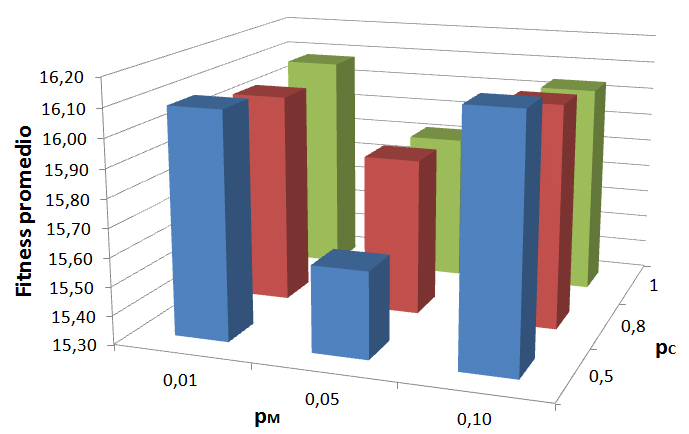
\includegraphics[width=0.8\linewidth]{Figures/grafica_mutacion_cruzamiento}
	\caption[Gráfica con combinaciones de probabilidad de cruzamiento y de mutación.]{Gráfica con combinaciones de probabilidad de cruzamiento (pc) y de mutación (pm).}
	\label{fig:grafica_mutacion_cruzamiento}
\end{figure}


Se comprueba que los resultados obtenidos siguen la distribución normal para poder aplicar el test de Student. 

%Siendo las hipótesis de la prueba u1 el promedio del  grupo 1 y u2 el del grupo 2)
%
%
%        \begin{equation}
%        \label{eq:student_eq}
%			\begin{split}
%				H0: u1  = u2  \\
%				H1: u1 != u2 
%			\end{split}			
%        \end{equation}

Si se compara la combinación del mejor promedio (0.5-0.1) y del peor (0.5-0.05) con el test de Student obtenemos t(x) = 0.07 que nos indica que para un nivel de significancia de  0,1 la hipótesis nula es rechazada, por lo tanto existe evidencia estadística para elegir la combinación con el mejor promedio (0.5-0.1) sobre la combinación con el peor promedio (0.5-0.05). Para comprobar si ésta es la mejor opción, se toman las dos combinaciones con el mejor promedio (0.5-0.1) y (0.5-0.01) obteniendo en el test Student t(x) = 0.71 que nos indica que no existe una diferencia significativa entre ambas muestras por lo que elegir una sobre otra no implicaría grandes beneficios. En tal sentido podríamos elegir cualquiera de las dos, en este caso se elige la combinación (0.5-0.01) por su buen promedio y baja desviación estándar.



\section{Descripción de escenarios}
Esta sección presenta los escenarios que serán evaluados experimentalmente. El primero es el escenario base que representa la realidad actual y el segundo es un escenario alternativo que presenta modificaciones respecto al caso base, con el objetivo de mejorar los resultados numéricos.

\subsection{Caso base o realidad actual del corredor}
El caso base representa la situación actual en términos de tráfico, red vial y sincronización de semáforos del corredor Garzón. Se simulan las instancias realistas desarrolladas en el capítulo 4 para obtener las velocidades promedio de ómnibus y otros vehículos y poder comparar con los resultados numéricos luego de aplicar el AE.  

Se realizó un estudio sobre datos proporcionados por la IMM que contenían el posicionamiento de los ómnibus, velocidad instantánea y datos de la línea durante todo el día para una semana en particular. De esta forma se constató que para las líneas de ómnibus que pasan por Garzón la velocidad promedio de los ómnibus es de 14.5 km/h. Esta información permitió calibrar el escenario modificando aspectos de la simulación relacionados con los ómnibus.

Sobre el escenario base geográfico se generan tres escenarios de tráfico : bajo, medio y alto. El caso medio representa los datos obtenidos en el trabajo de campo, el bajo es disminuyendo en un 50\% la cantidad de vehículos y disminuyendo el tiempo de espera en las paradas de ómnibus, teniendo en cuenta que en este caso existirán menos personas utilizando el transporte público. Las frecuencias de ómnibus se mantienen iguales ya que no son alteradas en la realidad cuando cambia la densidad de tráfico. El caso de tráfico alto se aumenta 50 \%  la cantidad de vehículos y el tiempo de espera en la parada de los ómnibus. El aumento y disminución del 50\% se obtuvo al analizar datos proporcionados por la IMM de la zona de Garzón de años anteriores. \newline

A continuación el resumen de la cantidad vehicular para los tres escenarios de tráfico:

\begin{itemize}
\item Tráfico Alto:  3000 vehículos en la simulación y 70 ómnibus. 
\item Tráfico Medio: 2000 vehículos y 70 ómnibus.
\item Tráfico Bajo:  1000 vehículos y 70 ómnibus.
\end{itemize}

 

\subsection{Escenario alternativo}

Para mostrar la utilidad que tienen las simulaciones de tráfico sobre un escenario que representa la realidad actual, se realiza un escenario alternativo. Una de las ventajas principales es que no requiere gran inversión monetaria, de tiempo y que no modifica la infraestructura del lugar, por lo que se pueden generar distintas pruebas para encontrar aquellas que logren un beneficio.

Analizando los puntos que se entienden podrían atentar contra el buen funcionamiento del Corredor, se agregan algunas modificaciones al escenario base para intentar mejorarlo. El objetivo no es encontrar la mejor alternativa, sino dar una de las muchas alternativas que se pueden generar y probar con las simulaciones de tráfico.
 % Ya que pueden existir limitaciones o reglas que no estamos tomando en cuenta y que deben cumplirse en la realidad.

Entre los cambios propuestos para el escenario alternativo se encuentran: eliminación de paradas y pasajes peatonales, alternancia de paradas y modificación de reglas de los semáforos.



\section{Resultados}
Esta sección muestra los resultados obtenidos tanto de la simulación de las instancias realistas desarrolladas, como de la aplicación del AE sobre las mismas. Se presenta la simulación del escenario alternativo y la posterior evaluación. Además se realizan estudios sobre cambios en la función de \emph{fitness} del AE y un breve análisis de la eficiencia computacional.


\subsection{Valores numéricos del caso base}

En la tabla \ref{table:resultado_caso_base} se pueden ver los resultados obtenidas para las diferentes instancias de tráfico simulado para el caso base. Estos datos representan la realidad actual del Corredor Garzón. Como se aprecia, la velocidad promedio de los ómnibus en tráfico medio es de 14.59 km/h, siendo 14.5 km/h el valor que se obtuvo de analizar los datos reales proporcionados por la IMM, lo que verifica que el modelo se aproxima a la realidad. 
 
 \begin{table}[H]
 	\renewcommand{\arraystretch}{1.2}
 	\caption[Resultados numéricos del caso base.]{Resultados numéricos del caso base, mostrando la velocidad promedio ómnibus (vpb) y velocidad promedio vehículos(vpv) para los distintos tipos de tráfico}
 	\label{table:resultado_caso_base}
 	\centering
 	\begin{tabular}{p{2.5cm}p{2.5cm}p{2.5cm}p{2cm} }
 		\hline
 		&
 		$vbp(km/h)$& 
 		$vvp(km/h)$ & 
 		Fitness \\ 
 		\hline
 		Tráfico Bajo & 15.89  & 32.45& 13.42\\
 		Tráfico Medio & 14.59  & 28.81& 12.05\\
 		Tráfico Alto & 14.31  & 26.36& 11.30\\

 		\hline
 	\end{tabular}
 \end{table}
 
 En el caso base no se calcula la desviación standard ya que los valores obtenidos son constantes (velocidad promedio de ómnibus, de otros vehículos y el valor de \emph{fintess}), pues siempre se simulan los mismos recorridos de los vehículos y la misma configuración de los semáforos. Cuando se aplica el AE, se generan nuevas configuraciones de semáforos, por lo que se obtiene un valor diferente de la velocidad promedio y del valor de \emph{fitness}, en este caso si se calcula la desviación standard.


\subsection{Resultados numéricos de la evaluación }

Como se aprecia en la tabla \ref{table:resultado_caso_algoritmo}, el AE mejora la velocidad promedio tanto de ómnibus como de otros vehículos en los tres tipos de tráfico estudiados. Además, la velocidad media de los vehículos se mantiene en un rango mucho más ajustado que en el caso original al variar el tráfico. Las mejoras logradas en el \emph{fitness} son de hasta 24\%. A continuación se describe el análisis estadístico para comprobar la mejora.


\begin{table}[H]
	\renewcommand{\arraystretch}{1.2}	
		\centering
	\caption[Resultados numéricos del AE]{Resultados numéricos del algoritmo evolutivo, mostrando velocidad promedio ómnibus (vpb) y de otros vehículos(vpv) para los distintos tipos de tráfico. }
	\label{table:resultado_caso_algoritmo}
	\begin{tabular}{cccccccc}
		\hline 
		Tráfico& 
		$vbp(km/h)$& 
		$vpv(km/h)$&
		\multicolumn{2}{c}{\emph{Fitness}}&  & 
		\multicolumn{2}{c}{Mejora \emph{fitness} (\%)}\\  \cline{4-5} \cline{7-8}&     &     & \multicolumn{1}{c}{Promedio} & \multicolumn{1}{c}{Mejor} &  & \multicolumn{1}{c}{Promedio} & \multicolumn{1}{c}{Mejor} \\ \hline
		Bajo & 17.92$\pm$0.18 & 34.30$\pm$0.40 & 14.50$\pm$0.14 & 14.88 & & 8.04 & 10.8  \\
		Medio& 16.95$\pm$0.32 & 33.29$\pm$0.29 & 13.95$\pm$0.15 & 14.19 & & 15.70& 17.7\\ 
		Alto & 16.51$\pm$0.61  & 32.90$\pm$0.25& 13.72$\pm$0.17 & 14.04 & & 21.40& 24.2\\	
		\hline	    
	\end{tabular}
\end{table}

Se realizaron 20 ejecuciones independientes del AE para cada tipo de tráfico, comprobando que los valores obtenidos siguieran una distribución normal. Por tanto se puede aplicar el criterio de significancia estadística para validar los resultados. Este criterio indica que el
algoritmo A es mejor que B si los resultados de A y B cumplen:

\begin{equation}
\label{eq:funcion_significancia}
\left |f_{avg}(A) - f_{avg}(B)  \right | > max(std(f_A),std(f_B))
\end{equation}

En este caso, A representa la aplicación del AE, y B el caso base. La Ecuación \ref{eq:funcion_significancia} indica que: el resultado promedio obtenido por el AE restado al valor del caso base, debe ser mayor a la máxima desviación standard calculada. Esta ecuación se cumple para todos los casos estudiados, por lo que se puede afirmar que existe evidencia estadística para afirmar que los resultados obtenidos por el AE son mejores a los valores del caso base.

\begin{figure}[H]
	\centering
	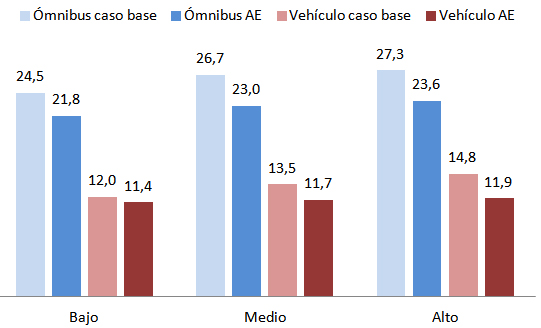
\includegraphics[width=0.8\linewidth]{Figures/duracion_viajes}
	\caption[Comparación de la duración en minutos de los viajes sobre el escenario base y al aplicar el algoritmo evolutivo.]{Comparación entre la duración en minutos de los viajes sobre el escenario base y al aplicar el AE al escenario alternativo, de ómnibus y otros vehículos en el recorrido completo del corredor Garzón para los diferentes tipos de tráfico.}
	\label{fig:duracion_viajes}
\end{figure}

En la Figura \ref{fig:duracion_viajes} se comparan las duraciones de los viajes obtenidas del caso base y las duraciones luego de aplicar el AE. Se comprueba que las duraciones de los viajes luego de aplicar el AE son menores tanto para ómnibus como para otros vehículos en los tres tipos de tráfico estudiados. 

%aprecia un resultado interesante, donde la duración original de los viajes cuando el tráfico es bajo es casi igual a la duración de los viajes con tráfico alto luego de ejecutar el AE. %Para ómnibus se tiene 24.5m y 23.6m y para otros vehículos 12.0m y 11.9m.

\subsection{Detalles del escenario alternativo}
Los cambios propuestos para el escenario alternativo incluyen eliminación de paradas, semáforos, pasajes peatonales y alternar paradas. Se estudiaron otras propuestas pero fueron descartadas por la poca viabilidad real de las mismas, como por ejemplo construir calles paralelas a Garzón o nuevas reglas en los cruces como existen en otros países.

\subsubsection{Eliminación de paradas}
Se consideraron eliminar dos paradas que cumplieran con las siguientes características: no estuvieran próximas a una calle principal y que existiera otra parada cercana para no afectar a los pasajeros realizando un traslado excesivo. Se seleccionaron las paradas ubicadas en las intersecciones de Garzón con las calles Ariel y Casavalle que cumplen con los criterios anteriores.

\subsubsection{Eliminación de pasajes peatonales}
Hay tres pasajes peatonales en el corredor Garzón con semáforos que detienen el tráfico, por lo tanto el objetivo al eliminarlos es aumentar la velocidad promedio de los vehículos circulantes . Dos de los pasajes peatonales controlan el flujo peatonal de las esquinas en la Plaza Vidiella y Camino Besnes e Irigoyen (sin pulsador en funcionamiento). En el escenario alternativo estos dos pasajes fueron cambiados por una señalización de \emph{pare} en la calle transversal al corredor Garzón. El tercer pasaje es netamente peatonal, y se encuentra ubicado frente a la Facultad de Agronomía, entre las calles Millán y Orticochea, el cual fue eliminado. Una opción para no eliminar físicamente los pasajes peatonales y mantener los resultados obtenidos, es implementar el pasaje peatonal por encima del corredor Garzón.

\subsubsection{Alternar paradas}

Uno de los problemas del ómnibus es su baja aceleración, por lo que cada vez que se detiene en un semáforo o en una parada, demora en retornar a una velocidad aceptable. Al reducir la cantidad de paradas donde un ómnibus tiene que detenerse se mejora la velocidad promedio.
La línea G recorre el corredor Garzón de punta a punta y es cubierta por las empresas Coectc y Cutcsa. Una posibilidad de alternancia de paradas consiste en dividir las paradas por empresa y compartir las ganancias del corredor u otro método para equiparar el pasaje transportado. 

\begin{figure}[H]
	\centering
	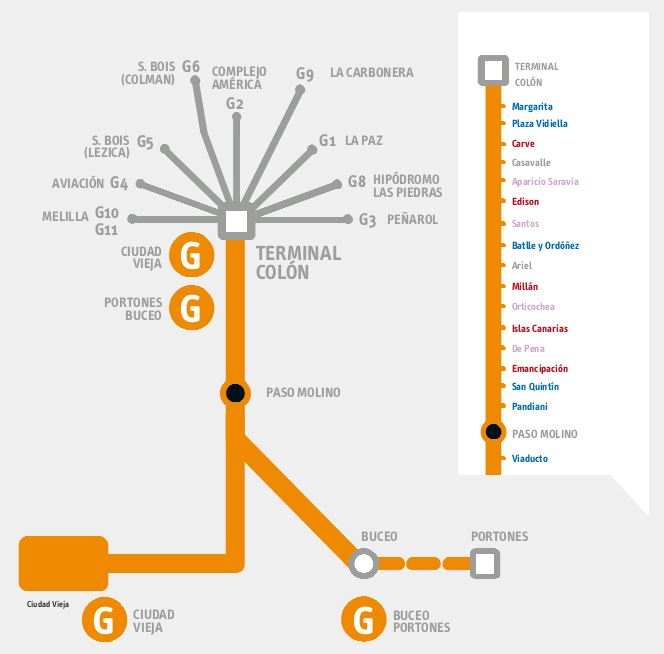
\includegraphics[width=0.9\linewidth]{Figures/paradas_alternativas}
	\caption[Gráfico de las paradas alternativas.]{Gráfico de las paradas alternativas. Gris: Parada Eliminada. Azul: línea G de Coectc y de Cutcsa. Rojo: línea G de Coectc. Violeta: G de Cutcsa. - Imagen original extraída de montevideo.gub.uy}
	\label{fig:paradas_alternadas}
\end{figure}

La Figura \ref{fig:paradas_alternadas} brinda un ejemplo donde, una empresa se detendrá en las paradas pares y la otra en las impares y algunas paradas con más cantidad de pasajeros serán realizadas por las dos. Cada empresa viajará por el corredor con una frecuencia de 4 minutos (como en la actualidad). Si se reduce el número de paradas donde se detiene un ómnibus, aumentará su velocidad promedio y no se deberá resentir en demasía el servicio ya que la disminución de la frecuencia en una parada se contrarresta con el aumento promedio de velocidad.

%El cambio de alternar paradas es el que más aumenta la velocidad media y tal vez es uno de los más sencillos de implementar en la realidad.


\subsubsection{Cambio básico de semáforos}
Al hacer el relevamiento de los datos obtenidos de la configuración de los semáforos del Corredor Garzón, se constató que en todas las intersecciones en donde una línea de ómnibus que circula por el corredor tiene un viraje a la izquierda, se hace detener el tránsito de la derecha de la misma, cada vez que el corredor central tiene la luz verde. Esto no parece tener mucho sentido ya que podrían seguir circulando por el corredor sin ningún tipo de problema. El carril que hay que detener es el de la izquierda del ómnibus cuando una línea dobla a la izquierda pero no los dos carriles al mismo tiempo. No se tiene conocimiento si corresponde a un error en la configuración, un tema de costos o facilidad para manejar los dos semáforos de los carriles paralelos juntos. Como esto ocurre en varias intersecciones y en ambos sentidos, el cambio mejora la velocidad promedio de los autos que circulan por los dos carriles.

Este cambio se aplicó en las siguientes intersecciones:
\begin{itemize}
	\item Islas Canarias: dobla línea 409 hacia la izquierda, orientado a Colón (Norte).
	\item Camino Ariel: doblan líneas como la  2 y la 148 hacia la izquierda, orientado a Paso Molino (Sur). 
	\item Camino Casavalle: dobla línea 174 hacia la izquierda, orientado a Paso Molino (Sur). 
\end{itemize}

\subsection{Valores numéricos al aplicar los cambios}

Para determinar cuales son los cambios que logran mejores rendimientos se elabora la Tabla \ref{table:resultado_alternativo}. Esta tabla se basa en el tráfico medio, ya que sólo se quiere realizar una comparación sencilla de las mejoras realizadas. Los cambios son acumulativos, por lo que se hacen uno después del otro. Se puede apreciar que la modificación que logra una mayor diferencia es la utilización de paradas alternadas.


\begin{table}[H]
	\renewcommand{\arraystretch}{1.2}
	\caption[Valores numéricos del escenario alternativo]{Valores numéricos del escenario alternativo con su velocidad promedio ómnibus (vpb) y velocidad promedio vehículos(vpv) comparando el \emph{fitness} para el tráfico medio }
	\label{table:resultado_alternativo}
	\centering
	\begin{tabular}{p{3.5cm}p{2.5cm}p{2.5cm}p{2cm}p{2cm} }
		\hline
		&
		$vbp(km/h)$& 
		$vvp(km/h)$ & 
		\emph{Fitness} &
		Mejora(\%)
		\\ 
		\hline
		Base & 14.59  & 28.81& 12.05 & -\\
		Eliminar Paradas & 15.44  & 29.03& 12.35 & 2.4\\
		Eliminar Peatonales  & 16.02  & 29.32& 12.59 & 4.4\\
		Paradas alternadas  & 19.17  & 28.88& 13.34 & 10.7\\	
		Cambio reglas  & 18.50  & 29.70& 13.39 & 11.1\\				
		\hline
	\end{tabular}
\end{table}

Una vez que se aplican todos las modificaciones sobre el escenario, se realiza un análisis para los demás tipos de tráfico. Como se ve en la Tabla \ref{table:mejoras_trafico_alternativo} se obtienen mejores rendimientos en todos los tipos de tráfico estudiados y el mejor rendimiento se obtiene cuando el tráfico es alto. 

\begin{table}[H]
	\renewcommand{\arraystretch}{1.2}
	\caption[Mejoras del escenario alternativo.]{Mejoras del escenario alternativo  para las velocidades promedio de los ómnibus(vpb) y de otros vehiculos (vpv) en el escenario alternativo para distintos tipos de tráficos }
	\label{table:mejoras_trafico_alternativo}
	\centering
	\begin{tabular}{p{3.5cm}p{2.5cm}p{2.5cm}p{2cm}p{2cm} }
		\hline
		&
		$vbp(km/h)$& 
		$vvp(km/h)$ & 
		Fitness &
		Mejora \emph{fitness}(\%)
		\\ 
		\hline

		Tráfico Bajo & 20.72  & 33.18 & 14.97 & 11.5\\
		Tráfico Medio & 18.50  & 29.70& 13.39 & 11.1 \\
		Tráfico Alto  & 18.60  & 27.17& 12.7 & 12.6\\		
		\hline
	\end{tabular}
\end{table}

Luego de obtener los valores para el escenario alternativo se procede a aplicarle el AE cuyo resultados veremos a continuación.


\subsection{Resultados de la evaluación sobre el escenario alternativo}

El escenario alternativo supuso una mejora sustancial en comparación con el caso base (11 \% en el valor de fitness). Se procede a aplicarle el AE para determinar si aún hay posibilidad de mejorar los valores de velocidad y \emph{fitness}.


Los resultados obtenidos en la Tabla \ref{table:mejoras_trafico_alternativo_algoritmo}  mejoran claramente el rendimiento del escenario alternativo y por supuesto del caso base en todos los tipos de tráfico. Comparando con la realidad actual se logran mejoras de hasta 37\%. 

Al comparar los resultados obtenidos se aprecia que cuanto mayor es la densidad de tráfico, mayor es el porcentaje de mejora. Además, un resultado interesante es que las diferencias entre los valores de los distintos tipos de tráfico se redujo.

\begin{table}[h]
	\renewcommand{\arraystretch}{1.2}
	\caption[Valores numéricos al aplicar el AE sobre el escenario alternativo.]{Mejoras obtenidas al aplicar el algoritmo evolutivo sobre el escenario alternativo, comparando las velocidades de ómnibus(vpb), otros vehículos(vpv) y el \emph{fitness} con cada tipo de tráfico contra el escenario base.}
	\label{table:mejoras_trafico_alternativo_algoritmo}
	\centering
	\begin{tabular}{cccccccc}
		\hline 
		Tráfico& 
		$vbp(km/h)$& 
		$vpv(km/h)$&
		\multicolumn{2}{c}{\emph{Fitness}}&  & 
		\multicolumn{2}{c}{Mejora \emph{fitness} (\%)}\\  \cline{4-5} \cline{7-8}&     &     & \multicolumn{1}{c}{Promedio} & \multicolumn{1}{c}{Mejor} &  & \multicolumn{1}{c}{Promedio} & \multicolumn{1}{c}{Mejor} \\ \hline

		Bajo & 23.15$\pm$0.36 & 34.43$\pm$0.33 & 15.99$\pm$0.08 & 16.10 & & 19.1& 19.90 \\
		Medio & 21.83$\pm$0.50  & 33.89$\pm$0.22 & 15.47$\pm$0.09& 15.65 & & 28.3 & 29.87\\
		Alto & 21.46$\pm$0.54  & 33.41$\pm$0.38 & 15.24$\pm$0.19& 15.50 & & 34.8 & 37.10\\	
		\hline		    
	\end{tabular}
\end{table}

En la gráfica de la Figura \ref{fig:duracion_viajes_alernativo} se comparan las duraciones de los viajes al aplicar el AE sobre el escenario alternativo. Se produce una gran reducción en la duración de los viajes de los ómnibus en los tres tipos de tráfico, mientras para el caso de los vehículos la mayor diferencia ocurre cuando el tráfico es alto.

\begin{figure}[H]
	\centering
	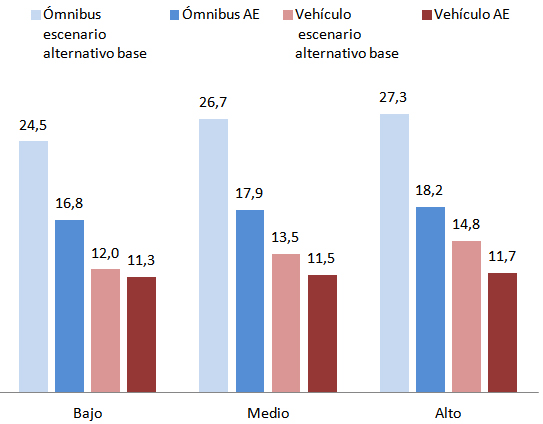
\includegraphics[width=0.8\linewidth]{Figures/duracio_viajes_alternativo}
	\caption[Comparación de la duración de los viajes en minutos entre el escenario base y el algoritmo evolutivo sobre el escenario alternativo.]{Comparación de la duración en minutos de los viajes realizados sobre el escenario base y al aplicar el algoritmo evolutivo  al escenario alternativo, de ómnibus y otros vehículos en el recorrido completo del corredor Garzón, para los diferentes tipos de tráfico.}
	\label{fig:duracion_viajes_alernativo}
\end{figure}

Otra vez se aplica el criterio de significancia estadística para comprobar que la mejora es significativa tanto al comparar con los valores del caso base como con los del escenario alternativo.

\subsection{Variación de la función de \emph{fitness}}

La función \emph{fitness} (\ref{eq:funcion_fitness}) utilizaba los pesos \emph{$w_1$ = $w_2$ = 1} lo que representa un balance equitativo para ómnibus y vehículos. Estos pesos pueden ser modificados en función de lo que se necesite, por lo que se realizaron pruebas con dos tipos de pesos para comparar como varían las velocidades cuando se da más peso a un tipo de vehículo sobre el otro.

%Por un cruce de Garzón pasan cada hora:
%70 ómnibus , si aproximamos con 23 personas= 1610 personas por hora
%800 autos, si aproximamos  2 personas por vehículo nos da 1600 personas por hora.
%Una cantidad similar  pasan por el cruce en ambos medios de transporte por lo que no existe una tendencia a favor de una sobre la otra, se podría aproximar que 50\% eligen el ómnibus y 50\% el auto.


\subsubsection{Prioridad ómnibus}
Este caso dará más prioridad a los ómnibus, este caso se justifica por el hecho que uno de los objetivos buscados por la IMM es que se utilice más el transporte colectivo como parte de su Plan de Movilidad Urbana. La premisa es que al mejorar la duración del viaje en ómnibus, en relación al del auto por el corredor, las personas que utilizan auto para sus viajes optarán por el transporte colectivo. Se experimentó cambiando los pesos de la función \emph{fitness} con un peso de 70\% para los ómnibus y 30\% al resto de los vehículos.


\subsubsection{Prioridad a otros vehículos}

Este caso asigna 70\% del peso a los vehículos y 30\% a los ómnibus. Es el caso opuesto al anterior y resulta útil para poder comparar como varían los valores de las velocidades.

\subsubsection{Resultados}

La Tabla \ref{table:analisis_fitness} compara las velocidades promedio de ómnibus y vehículos para los tres tipos de pesos que se probaron y por cada tipo de tráfico.  El caso 50-50 es el caso base donde los pesos son iguales, 70-30 es el caso con más prioridad para los ómnibus y el 30-70 más prioridad a los otros vehículos. Se analiza cuanto varían las velocidades de ómnibus (var. vpb) y otros vehículos(var. vpv) comparando contra el caso 50-50 de cada tipo de tráfico.


\begin{table}[H]
	\renewcommand{\arraystretch}{1.2}
	\caption[Valores obtenidos al modificar los pesos de la función de \emph{fitness}.]{Valores obtenidos al modificar los pesos de la función de \emph{fitness}, analizando las variaciones en la velocidad promedio de ómnibus (vpb), otros vehículos (vpv) y \emph{fitness}. }
	\label{table:analisis_fitness}
	\centering
	\begin{tabular}{p{1cm}p{1.2cm}p{1.8cm}p{1.8cm}p{1.8cm}p{1.2cm}p{1.2cm}p{1.2cm} }
		\hline
		Tráfico &
		pb(\%) pv (\%)& 
		vpb & 
		vpv &
		fitness &
		var. \newline vpb(\%) &
		var. \newline vpv(\%) &
		var. \newline \emph{fitnesss}(\%)
		\\ 
		\hline
		& 50-50  & 17.92$\pm$0.18 & 34.30$\pm$0.40 & 14.50$\pm$0.14  &- & - & -\\		
		Bajo & 70-30  & 17.93$\pm$0.23 & 34.06$\pm$0.17 & 12.65$\pm$0.11  & +0.07 & -0.70 & -12.79\\		
		& 30-70 & 17.55$\pm$0.23 & 34.71$\pm$0.21 & 16.42$\pm$0.10  & -2.06 & +1.18 & +13.21\\
		\hline
		
		& 50-50  & 16.95$\pm$0.32 & 33.29$\pm$0.29 & 13.95$\pm$0.15  &- & - & -\\		
		Medio & 70-30  & 17.29$\pm$0.27 & 33.08$\pm$0.14 & 12.24$\pm$0.12  & +2.0 & -0.62 & -12.30\\		
		& 30-70 & 16.71$\pm$0.42 & 33.79$\pm$0.31 & 15.92$\pm$0.11  & -1.41 & +1.49& +14.11\\
		
		\hline
		& 50-50  & 16.51$\pm$0.60 & 32.90$\pm$0.25 & 13.72$\pm$0.17  &- & - & -\\		
		Alto & 70-30  & 16.72$\pm$0.14 & 32.79$\pm$0.26 & 13.75$\pm$0.07  & +1.24 & -0.33 & +0.19\\	
		& 30-70 & 15.48$\pm$0.42 & 33.20$\pm$0.25 & 15.49$\pm$0.16  & -6.23 & +0.92 & +12.87\\
		\hline
	\end{tabular}
\end{table}


Los resultados indican que al variar los pesos de la función \emph{fitness} las velocidades promedio de los vehículos se ve afectada. Al dar más prioridad a los ómnibus se produce, como cabía esperar, un aumento en su velocidad promedio y una leve baja en la velocidad promedio del resto de los vehículos. Cuando el tráfico es bajo este cambio casi no aumenta la velocidad de los ómnibus. Una explicación posible de este comportamiento es que ya se llegó a un limite máximo y no se puede mejorar más.

Al dar más prioridad a los otros vehículos se produce un aumento en su velocidad y una disminución en la velocidad de los ómnibus la cual es muy evidente en el caso de tráfico alto. Este resultado permite apreciar como estos valores son fuertemente afectados por la densidad de tráfico que se estudie.

En general las variaciones en las velocidades no son grandes, pero suficientemente apreciable para tener cierta libertad al plantear distintos objetivos que tiendan a favorecer un tipo u otro de vehículos.


\subsection{Eficiencia computacional}

Se realiza un estudio de la eficiencia computacional del AE para analizar los tiempos de ejecución cuando se usan varios procesadores y como se desempeña su capacidad de paralelismo.

Se evalúan nueve ejecuciones del AE; tres con cada tipo de tráfico: alto, medio y bajo, para estudiarlo en diferentes contextos. El algoritmo utiliza 32 hilos de ejecución por lo que utilizamos esa cantidad de núcleos.

Las pruebas fueron realizadas sobre el node40 del Cluster Fing, con un procesador AMD Opteron 6272 2.09GHz, 48 GB RAM y 32 núcleos utilizados.

El \emph{speedup} (S) mide la mejora de rendimiento de una aplicación al aumentar la cantidad de procesadores comparando con el rendimiento al usar un solo procesador.
\begin{equation}
\label{eq:funcion_speedup}
S = \frac{T_1}{T_N}
\end{equation}
Donde ${T_1}$ es el tiempo de ejecución del algoritmo serial o secuencial, y ${T_N}$ el tiempo del algoritmo ejecutado sobre N procesadores.
\newline

La eficiencia computacional (E) corresponde al valor normalizado del \emph{speedup} (entre 0 y 1) respecto a la cantidad de procesadores. Los valores cercanos a uno indican una alta eficiencia computacional.
\begin{equation}
\label{eq:funcion_eficiencia}
E = \frac{T_1}{N*T_N} = \frac{S}{N}
\end{equation}



\begin{table}[H]
	\renewcommand{\arraystretch}{1.2}
	\caption[Análisis de la eficiencia computacional.]{Análisis de la eficiencia computacional comparando los tiempos de ejecución en serial y paralelo en minutos. }
	\label{table:analisis_speedup}
	\centering
	\begin{tabular}{p{2.5cm}p{2.5cm}p{2.5cm}p{2.5cm}p{2.5cm} }
		\hline
		
		Instancia& 
		Serial(m) & 
		Paralelo(m) &
		\emph{Speedup} &
		Eficiencia
		\\ 
		\hline
		bajo1  & 1572 & 59 & 26.64 & 0.83\\
		bajo2  & 1571 & 59 & 26.62 & 0.83\\
		bajo3  & 1183 & 44 & 26.88 & 0.84\\
		
		medio1  & 3002 & 119 & 25.22 & 0.78\\
		medio2  & 2195 & 82 & 26.76 & 0.83\\
		medio3  & 3007 & 120 & 25.05 & 0.78\\
		
		alto1  & 2920 & 110 & 26.5 & 0.82\\
		alto2  & 4365 & 183 & 23.85 & 0.74\\
		alto3  & 4276 & 177 & 24.15 & 0.75\\
		\hline
		  &  & Promedio & 25.7$\pm$1.1 & 0.80$\pm$0.03\\
		
		\hline
	\end{tabular}
\end{table}

 Tabla \ref{table:analisis_speedup} El algoritmo paralelo logra una mejora sustancial en los tiempos de ejecución con un valor promedio del \emph{speedup} de 25.7  y  eficiencia promedio de 0.8, lo cual puede considerarse como buenas métricas.

\begin{figure}[H]
	\centering
	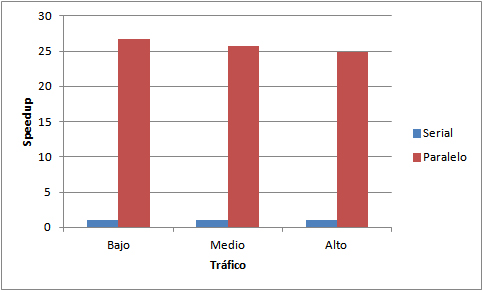
\includegraphics[width=0.8\linewidth]{Figures/speedup1}
	\caption[Comparación de los \emph{speedup} promedios para cada tipo de tráfico.]{Comparación de los \emph{speedup} promedios para cada tipo de tráfico. Se representa el caso serial que corresponde al \emph{speedup} = 1 para fines de comparación.}
	\label{fig:speedup1}
\end{figure}

La gráfica de la Figura \ref{fig:speedup1} muestra como al aumentar el tráfico disminuye el \emph{speedup}. Este fenómeno sucede porque está influenciado por los accesos al disco duro, al tener más vehículos circulando en la simulación se tiene que leer y escribir más información en los archivos, lo que aumenta el tiempo de ejecución del algoritmo (aunque como se ve no tiene un gran impacto).